\chapter{REVISÃO DE LITERATURA}
\label{chp:capitulo2}

Em um campo com uma quantia tão rarefeita de artigos, publicações e materiais em larga parte espalhadas por blogs na internet, foi necessário realizar uma revisão de literatura para que as ferramentas de ponta, estratégias ainda sendo testadas e vulnerabilidades principais no mercado fossem corretamente identificadas. Isso se torna especialmente verdadeiro pela mudança no cenário de segurança dos anos 2000 para os anos 2010-2022, aonde boa parte de ameaças antigas podem ser de pouca relevância.

Aqui serão amostrados alguns dos principais achados, as estratégias para organizar os mesmos e resumido o estado da arte no presente momento.

\section{Levantamento de Artigos}

Para a coleta e organização de artigos em si, as principais utilidades empregadas foram o Parsifal, o Scopus e o CAFe (disponibilizado pela Universidade Federal do Rio de Janeiro). 

\subsection{Parsifal}
Parsifal é uma ferramenta originalmente designada para realizar Revisões Sistemáticas de Literatura, que embora sejam de escopo maior que a revisão rápida que foi realizada neste trabalho, ainda contou com uma série de funcionalidades que permitisse catalogar, processar e essencialmente medir o progresso das pesquisas realizadas no assunto.

\begin{figure}[ht]
    \centering
    \caption{Dashboard Parsifal}
    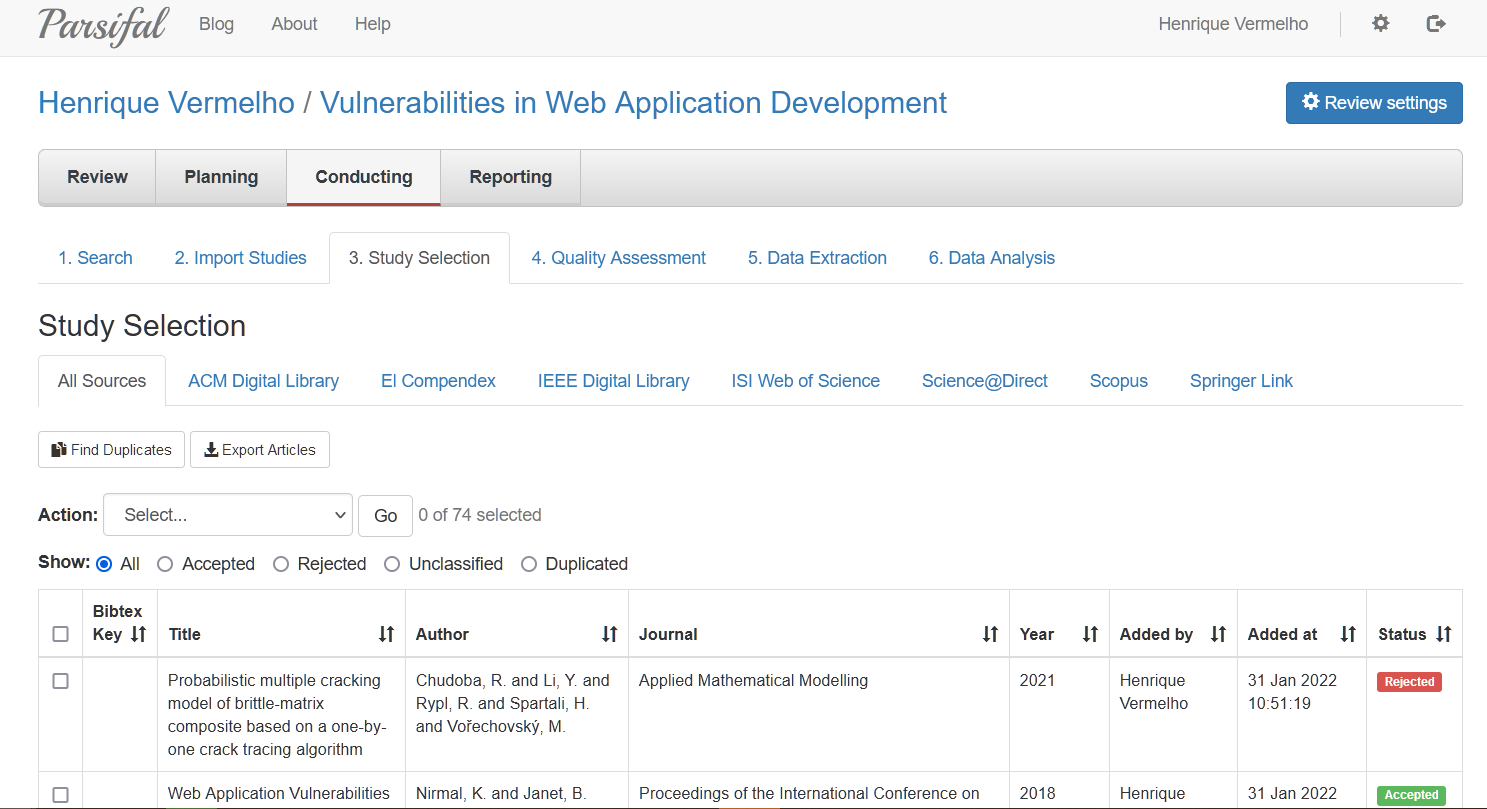
\includegraphics[width=14cm]{figuras/parsifal.png} 
    \legend{Fonte: \href{https://parsif.al}{parsif.al} (2022, p. TO-DO)}
    \label{fig:internet} 
\end{figure}

\bigskip

Na figura acima pode-se verificar no topo quatro abas principais - \textbf{Review, Planning, Conducting, }e \textbf{Reporting}. A primeira é simples e não muito essencial, descrevendo apenas os colaboradores registrados na plataforma na determinada pesquisa. A segunda, no entanto, é composta de três etapas interdependentes:

\begin{alineas}

\item \textbf{Protocol} - estabelece os objetivos, e parâmetros da pesquisa. Tais parâmetros chaves incluem PICOC (population, intervention, comparison, outcomes and context - fatores que permitem sondar o objetivo), Research Questions, Keywords + Sinônimos, Search String, Buscas e Critério de Seleção.

\item \textbf{Quality Asessment Checklist} - o pesquisador estabelece uma série de perguntas sobre os artigos, e a resposta para essas (Sim, Parcialmente, Não no caso dessa pesquisa) recebe um peso que permite classificar um artigo como aceito ou rejeitado na seleção final. 

As perguntas escolhidas priorizavam bons resultados descritos nos artigos, artigos na língua inglesa, problemas abertos, contexto de aplicações web e papers com download/visualização disponíveis (uma dificuldade que será discutida mais a frente).

\item \textbf{Data Extraction Form} - Permite nomear agrupar dados de destaque de artigos aceitos.

\end{alineas}

A etapa seguinte, a de \textbf{Conducting}, é um tanto mais complexa composta de mais subetapas. São elas:
\begin{alineas}
\item \textbf{Search} - verifica-se a Search String definida na etapa anterior de Planning. No final optou-se por ("Web Apps" OR "Web Application") AND ("Hardening") AND ("Prevention" OR "Avoidance") AND ("Secure Coding") AND ("Vulnerability").

\item \textbf{Import Studies} - nessa subetapa há a opção de importar para a plataforma metadados das publicações encontradas (studies), no formato \textit{BibTeX}. Ao total foram em torno de 74 artigos selecionados para avaliação, todos oriundos do Scopus que será descrito a seguir.

\item \textbf{Study Selection} - uma das partes mais importantes - é realizada a seleção dos artigos, além da eliminação dos artigos duplicados na busca. É a seção amostrada na captura de tela acima. Uma série de metadados é mostrada e é possível filtrar por fonte, artigos aceitos, rejeitados, duplicados e ainda não classificados.

\item \textbf{Quality Assessment} - as perguntas criadas na subetapa Quality Assessment Checklist da etapa anterior de Planning são respondidas aqui, o que determina o aceite ou não de determinados artigos baseados em suas "pontuações" por perguntas respondidas.

\item \textbf{Data Extraction} - é feita a anotação de acordo com os grupos denominados na etapa anterior pelo pesquisador. Porém não foi muito utilizada no escopo deste trabalho.

\item \textbf{Data Analysis} - como o nome descreve, o Parsifal disponibiliza nessa subetapa uma série de gráficos a respeito dos dados trabalhados. São eles: artigos por fonte, artigos aceitos por fonte, e artigos por ano dentre os aceitos. Os resultados dessa seção estão contidos nos apêndices.

\end{alineas}

Por fim, há a etapa final \textbf{Reporting}, que é permite ao pesquisador exportar um relatório final com os principais resultados do Parsifal - selecionando os dados desejados. Esse relatório encontra-se nos apêndices.

\subsection{Scopus + CAFe},
O Scopus é o banco de dados disponibilizado pela Elsevier de citações e abstracts.

TO-DO printscreen do Scopus. CAFe. Dificuldades encontradas. (artigos não baixáveis etc) cafe bugado

\section{nscanner}

\section{WAF-A-MoLE}

\subsection{Linear SVM}

\subsection{Seção Terciária}

Alíneas e subalíneas.
\bigskip

\begin{alineas}
\item linha 1:
\begin{alineas}
\item subalinea 1;
\item subalinea 2;
\end{alineas}
\item linha 2:
\begin{subalineas}
\item subalinea 1;
\item subalinea 2;
\end{subalineas}
\item linha 3:
\begin{incisos}
\item subalinea 1;
\item subalinea 2;
\end{incisos}
\item linha 4.
\end{alineas}

